%%
%% paper.tex — Intelligent Motion Control of BUV
%% Сохранять в кодировке CP866 !!!
%%
\documentclass[12pt]{revtex4}
\usepackage{graphicx}  
\begin{document}

\title{Intelligent Motion Control of an Underwater Biomimetic Robot
       Using Deep Reinforcement Learning}

\author{G.V. Kazantsev}
\author{L.A. Stankevich}
\affiliation{Central Research and Development Institute of Robotics
             and Technical Cybernetics, Saint-Petersburg, Russia}

\date{\today}

\begin{abstract}
Control of biomimetic underwater vehicles (BUVs) is complicated
by the nonlinearity of hydrodynamics and the lack of accurate
analytical models, which limits the application of classical
controllers. This paper proposes a control system for a robotic
fish with a multi-link caudal fin based on deep reinforcement
learning without explicit hydrodynamic modeling. The problem is
formalized as a Markov decision process and solved using the
Soft Actor-Critic (SAC) algorithm with a multi-component reward
function in the Stonefish~2 simulator integrated with ROS2.
Experimental results demonstrate that the trained policy achieves
a steady-state depth error of 0.07\,m with a standard deviation
of 0.04\,m, a settling time of 22\,s, and a maximum velocity of
0.15\,m/s while maintaining heading. The results confirm the
effectiveness of the proposed approach for developing adaptive
control systems for biomimetic underwater vehicles.

\medskip
\noindent\textbf{Keywords:} intelligent control systems,
biomimetic underwater vehicles, deep reinforcement learning,
Soft Actor-Critic (SAC), ROS2, hydrodynamic simulation.
\end{abstract}

\maketitle

% ================== SECTION 1 ==================
\section{Introduction}


Biomimetic underwater vehicles (BUVs) have attracted considerable interest due to their potential utility in aquatic missions. The biomimetic design of such vehicles enables locomotion through interaction with the surrounding environment. These vehicles are capable of utilizing water energy significantly more efficiently compared to conventional axial propellers and are also characterized by reduced noise. By replicating the movements of marine fauna, in particular the undulatory motions of the tail or the entire body, BUVs achieve energy-efficient motion and enhanced maneuverability.

One of the promising tasks in robotics is the development of robotic fish capable of navigating in complex aquatic environments, including confined and hard-to-reach spaces comparable to the robot's own dimensions [1]. Such tasks arise in coral reef exploration, inspection of sunken objects, seabed surveys, underwater pipeline and structure inspection, as well as aquaculture monitoring and ecological studies in enclosed water bodies [2]. Robotic fish represent a promising solution for aquatic tasks, offering several advantages over conventional unmanned underwater vehicles (UUVs), including maneuverability in constrained conditions, high energy efficiency, reduced detectability, and minimized mechanical impact on the environment.

The interaction of the robot with the environment is described by hydrostatic, hydrodynamic, control forces, and moments. Hydrostatic forces include residual buoyancy, which describes the difference between the actual buoyancy reserve and the calculated one, as well as longitudinal and transverse stability moments. Hydrodynamic effects include viscous drag forces and inertial forces due to added fluid masses. Hydrodynamic forces also depend on the body shape and the flow regime, characterized by the Reynolds number [3].

Among the key challenges in developing biomimetic underwater vehicles - the design of efficient propulsors, control algorithms, and navigation systems - the central problem is the synthesis of a robust control law. This is due to the fact that the vehicle dynamics represent a nonlinear, multidimensional system operating under uncertainty and in the absence of an accurate mathematical model. The solution to this problem appears to lie in the use of hybrid intelligent control systems combining classical control theory methods with reinforcement learning algorithms for adaptation to changing environmental conditions.

The main contribution of this work is: 1) the development of a multi-component reward function that simultaneously stabilizes depth and heading while maximizing the cruising speed of the BUV without constructing an explicit hydrodynamic model; 2) experimental justification of the necessity of using a stack of five previous observations to compensate for the time delay in the buoyancy control channel; 3) the creation of a scalable software architecture with parallel training environments based on Docker and Kubernetes, ensuring reproducibility of experiments and a throughput of approximately 1000 simulation steps per second.

The practical significance of this work lies in the applicability of the developed algorithms and software tools for building autonomous control systems for biomimetic underwater vehicles across a wide range of tasks: environmental monitoring of water bodies, inspection of underwater structures, aquaculture monitoring, and search operations under complex hydrodynamic conditions.

The remainder of this paper is organized as follows. Section II presents a literature review on the control of conventional and biomimetic robots. Section III describes the prototype robot design, its model in the Stonefish simulator, and the formulation of the deep reinforcement learning problem. Simulation results are presented in Section IV. Conclusions and directions for future research are discussed in Section V.

% ================== SECTION 2 ==================
\section{Related Work}


Vehicle propulsion in a fluid can be achieved through one of several fundamental methods: using propellers, through body shape changes, using jet propulsion, or through the action of internal mechanisms. Traditional autonomous unmanned underwater vehicles (AUVs) have achieved significant success in exploring the underwater domain precisely due to propeller-type thrusters. An example is the deep-water vehicle Vityaz-D, developed at the Rubin Central Design Bureau (Russia). This robot, whose external appearance is shown in Fig.~\ref{fig:vehicles}, is capable of diving to a depth of 11,000 meters and addressing a wide range of scientific and applied tasks - from marine biology to geological surveys. Motion control of the  Vityaz-D is performed by means of main and maneuvering propellers, while course and depth correction is achieved using control surfaces. The vehicle's navigation system integrates data from an inertial measurement unit, a Doppler velocity log, and hydroacoustic sensors [5]. The control system software features a multi-level architecture: the lower level, based on PID controllers, is responsible for stabilizing heading, roll, and pitch, while the upper level provides route planning, obstacle avoidance, and response to emergency situations.

In recent years, considerable interest has emerged in small-sized mobile robots employing an alternative locomotion method - changing the shape of the body and fins. In fish-like robots, there are more than ten such methods, determined by the nature of the wave motion of the body or fins [4]. Locomotion in this case is based on the physical properties of fluid viscosity and the associated processes of vortex formation [5].

Among the diversity of biomimetic vehicles, several characteristic approaches to control system design can be distinguished. The control system of the manta ray robot [6] is built on central pattern generators with Hopf oscillators controlling five servo drives. The stable limit cycle ensures smooth transitions between modes without signal discontinuities; however, feedback is implemented only through sensors, and self-learning and adaptive policy are absent.

A more complex architecture is demonstrated by the underwater snake robot EELUME [7], whose control system has a three-level structure: a motion planning level, a level for calculating control forces and moments, and a level for distributing thrust among the thrusters considering the current joint configuration. In the transportation mode, the integral line-of-sight (ILOS) method is used, generating a reference heading based on the cross-track error with integral compensation for constant current; the joints are then deflected according to a PID law proportional to the heading error. In the working mode, the robot acts as a floating manipulator with task prioritization and avoidance of singular configurations. This approach requires an accurate hydrodynamic model and manual tuning of controllers, which limits adaptability under non-stationary conditions.

Among fish-like robots, three representative examples also stand out. The BUV prototype from Immanuel Kant Baltic Federal University and Nizhny Novgorod State University [1] with a thunniform propulsor employs spiking neural networks. A high-speed tuna robot [8], achieving 4.3 body lengths per second, is controlled by a PID regulator maintaining the tail frequency and amplitude. A robot with a soft silicone tail [9] uses an adaptive controller based on the support vector machine method to stabilize velocity under variable loads. Despite the diversity of the listed approaches, all of them either do not provide adaptation to a changing environment or require an accurate analytical model, which motivates the transition to reinforcement learning methods.


A number of recent works confirm the effectiveness of reinforcement learning for BUV control. In [10], a controller is trained using the SAC algorithm in the FishGym environment, while a second module predicts flow parameters, enabling the robot to adapt to currents not encountered during training. In [11], SAC is augmented with HER and CQL methods for path planning with obstacles without a prior environment map. In [12], a PPO algorithm trained directly on a physical robot reached target points within 50,000 steps; however, prolonged training led to servo drive wear, confirming the necessity of the sim-to-real strategy adopted in the present work.

Article [13] classifies RL environments into three levels of complexity: for fast simulations, on-policy PPO is preferable, whereas for real robots, off-policy methods (SAC, DDPG, TD3) are more advantageous as they utilize training examples more efficiently. The existing MarineGym environment is designed for propeller-type thrusters and is unsuitable for the undulatory locomotion of BUVs. Hybrid MPC+RL approaches are limited by the need for an accurate model and high computational costs.

A comparative analysis of known algorithms (PPO, SAC, TD3, MPC+RL) in terms of implementation complexity, training speed, solution quality, adaptability, and stability shows that the SAC algorithm demonstrates the best balance between training speed, solution quality, and stability. Unlike MPC+RL, SAC does not require an explicit specification of the vehicle's dynamic and hydrodynamic model; compared to PPO, SAC is an off-policy method, which provides higher efficiency in utilizing training examples - a critical advantage when working with a computationally expensive hydrodynamic environment. The combination of these factors determined the choice of SAC as the primary reinforcement learning algorithm in the present work.


% ================== SECTION 3 ==================
\section{Robot Model and Simulation Environment}


The BUV prototype developed at the Central Research and Development Institute of Robotics and Technical Cybernetics (Saint-Petersburg), shown in Fig.~\ref{fig:cad_model}, is used as the base model for this study. The prototype was successfully tested for watertightness and overall structural integrity, confirming its ability to perform translational motion underwater and execute basic maneuvers, including course changes and depth adjustment in manual control mode. The prototype was also equipped with three cameras, a water acidity sensor, a water temperature sensor, and a pressure sensor for measuring water characteristics. 
Final technical specifications of the vehicle, obtained after several 
stages of field testing, are as follows: weight --- 1.5 kg; overall 
dimensions (L $\times$ W $\times$ H) --- 430 $\times$ 215 $\times$ 120 mm; 
average speed --- 0.05 m/s; maximum speed (experimental) --- 0.14 m/s; 
maneuverability (yaw angular velocity) --- 8.2$^\circ$/s; biomorphic 
propulsor design.

The design of the biomimetic propulsor is shown in Fig.~\ref{fig:prototype}. It is located in the tail section of the robot and consists of a brushless motor with a gearbox, a crank-slider mechanism, a servo drive with an eccentric, and a flexible caudal fin. Torque from the motor is transmitted to the eccentric, which moves the carriage along aluminum tube guides, converting rotary motion into reciprocating motion and then into oscillatory motion of the tail.

The digital model of the robotic fish, in turn, incorporates a geometrically simplified body and fin geometry, streamlined for computation. The original model contained fastening elements (screws, clamps, mounting and fastening holes) and electronics, which were removed to obtain a smooth body surface and reduce the number of finite-element mesh nodes. To compensate for the mass of the removed elements, point masses were added at the corresponding locations of the simplified model, allowing the original center of mass position to be preserved unchanged relative to the full model. This simplification reduced the computational load without introducing significant errors into the hydrodynamic analysis results, since the removed elements do not significantly affect the flow around the body [14], and their inertial characteristics are accounted for through the point masses. The body material in the simulation is assigned properties corresponding to ABS plastic with a density of 1.04~g/cm$^3$.

The choice of simulation environment determines the feasibility and quality of the research, as well as the possibility of subsequently transferring the algorithms to the real prototype. Two key requirements are imposed on the environment: high fidelity of hydrodynamic process modeling and built-in support for reinforcement learning interfaces. The NVIDIA Isaac Sim and MuJoCo packages, although possessing high computational speed and built-in GPU computation support, require high-performance hardware for hydrodynamic calculations, which lack native support and require the development of additional modules implementing fluid physics. The Ansys Fluent package, being a benchmark for computational fluid dynamics (CFD), is entirely unsuitable for iterative neural network training due to its low simulation speed.

Preliminary simulations revealed that using a rigid tail consisting of a single segment does not allow the vehicle to perform translational motion underwater. Instead of generating thrust, only rocking of the vehicle's body in place occurs. To solve this problem, a modified tail assembly model was developed, consisting of five dependent rigid links connected by revolute joints (Fig.~\ref{fig:tail}). This approach approximates the bending wave characteristic of this type of locomotion. To simplify the control action and focus the research on high-level control algorithms rather than searching for low-level patterns, a sinusoidal locomotion model is used for the deflection angles of each of the five links.

The kinematics of the tail are described by a traveling wave model. The amplitude increases linearly from head to tail with coefficients $g_i = [0.2, 0.4, 0.6, 0.8, 1.0]$. The angular position of the $i$-th joint at time $t$ is given by the equation:
\[
\theta_i(t) = A_{\max} \cdot g_i \cdot \sin(2\pi f t - k \frac{i}{N}) + B_i \cdot \phi,
\]


\noindent where $\theta_i(t)$ is the rotation angle of the $i$-th joint; $A_{max}$ is the maximum amplitude; $f$ is the undulation frequency; $k$ is the wave number; $\phi$ is the asymmetry for heading control; $B_i$ is the influence coefficient of the offset on the $i$-th joint; $N$ is the number of tail segments.

Differentiating with respect to time yields the expressions for angular velocity and angular acceleration of the joints:
\[
\dot{\theta}_i(t) = \frac{d\theta_i}{dt} = 2\pi f \cdot A_{\max} \cdot g_i \cdot \cos\left(2\pi f t - k \frac{i}{N}\right),
\]

\[
\ddot{\theta}_i(t) = \frac{d^2\theta_i}{dt^2} = -(2\pi f)^2 \cdot A_{\max} \cdot g_i \cdot \sin\left(2\pi f t - k \frac{i}{N}\right),
\]

\noindent where $\dot{\theta}_i(t)$ is the angular velocity of the $i$-th joint; $\ddot{\theta}_i(t)$ is the angular acceleration of the $i$-th joint.

The maximum values of velocity and acceleration are reached when $\cos(\cdot)$ and $\sin(\cdot)$ equal $\pm 1$:

\[
\dot{\theta}_{i,\max} = 2\pi f \cdot A_{\max} \cdot g_i,
\]

\[
\ddot{\theta}_{i,\max} = (2\pi f)^2 \cdot A_{\max} \cdot g_i.
\]

Considering the physical limitations of the tail construction, the limiting values of amplitude and frequency are chosen from the conditions:

\[
\dot{\theta}_{i,\max} < \dot{\theta}_{\max,\text{servo}},
\]

\[
\ddot{\theta}_{i,\max} < \ddot{\theta}_{\max,\text{servo}}.
\]

The dynamics of the robotic fish are computed using the Bullet Physics library with the Featherstone algorithm [15] for articulated body systems, enabling the calculation of the kinematics of the robot's multi-link caudal fin. Hydrodynamic forces are computed using the finite element method, eliminating the need for simplified analytical approximations for bodies of complex shape. The buoyancy force is calculated by integrating the hydrostatic pressure over all submerged faces. This approach ensures high accuracy at the interface between media (e.g., during partial surfacing with consideration of waves). The drag force is the sum of the quadratic form drag [16]:

\[
d\mathbf{F}_{\text{form}} = -\frac{1}{2} \rho C_d |\mathbf{V}_{\text{flow}} \cdot \mathbf{n}| (\mathbf{V}_{\text{flow}} \cdot \mathbf{n}) \mathbf{n} \, dA,
\]

\noindent where $\rho$ is the fluid density; $C_d$ is the form drag coefficient, which may depend on the material and local geometry; $|\mathbf{V}_{\text{flow}} \cdot \mathbf{n}|$ is the scalar projection of the relative velocity onto the normal; $(\mathbf{V}_{\text{flow}} \cdot \mathbf{n})$ is the magnitude of the projection of the relative velocity onto the normal; $dA$ is the area of the mesh finite element,

\noindent and viscous friction [16]:

\[
d\mathbf{F}_{\text{visc}} = -\frac{1}{2} \rho C_f |\mathbf{V}_{\text{flow}}| \mathbf{V}_{\text{tang,flow}} \, dA,
\]

where $C_f$ is the viscous friction coefficient; $\mathbf{V}_{\text{tang,flow}}$ is the tangential component of the relative flow velocity.
The applied approach, based on calculating forces for local surface elements, allows for qualitative modeling of the robot's interaction with the flow while avoiding the computational complexity of a full-fledged CFD solution of the Navier-Stokes equations in real time.

Since the Stonefish simulator uses a simplified discrete hydrodynamic model, it is necessary to verify the adequacy of the modeling for the specific geometry of the biomimetic robot. To validate the dynamic characteristics of the digital model, test simulation runs were conducted. The experiment involved measuring the steady-state horizontal velocity of the robot at a fixed depth of 2 meters and constant undulation parameters of the caudal fin (sinusoidal motion law for 5 rigid links). The results were compared with the tactical and technical characteristics of the prototype provided in the previous section.

At a constant specified tail oscillation frequency of 0.3 Hz at a depth of 2 meters, the steady-state horizontal velocity was 0.015 m/s. In turn, for a frequency of 3 Hz, the fish velocity was 0.2 m/s, which coincides within the margin of error with the technical characteristics of the developed fish prototype. The simulation environment qualitatively demonstrates the behavior of the underwater vehicle. Figure~\ref{fig:sim_models} shows the robot representations used in the simulation: 1 - hydrodynamic model (finite-element mesh of faces); 2 - geometric 3D model; 3 - collision model for collision calculations in Bullet Physics; 4 - kinematic model of the tail consisting of 5 rigid links.

To solve the formulated control problem, the SAC algorithm proposed by Haarnoja in [17] and implemented in the Stable-Baselines 3 library was selected. Unlike algorithms of the DQN family, SAC is capable of operating with continuous control signals, which eliminates the need for discretization and the associated loss of control precision. SAC is an off-policy algorithm that uses an experience replay buffer. This becomes important for solving the problem at hand, since collecting a single episode in a hydrodynamic simulator requires significant computational resources, and reusing data accelerates convergence [18].

The central idea of SAC, distinguishing it from other algorithms, 
is the maximization of not only the expected return (discounted sum 
of rewards) but also the entropy of the policy. This is expressed in 
the following objective function:

\[
J(\pi) = \sum_{t=0}^{T} \mathbb{E}_{(s_t, a_t) \sim \rho_\pi} \left[ R(s_t, a_t) + \alpha \mathcal{H}(\pi(\cdot|s_t)) \right],
\]

where $J(\pi)$ is the objective function for optimization; $\pi$ is the agent's policy; $\rho_\pi$ is the distribution of states and actions under the policy; $R(s_t, a_t)$ is the reward obtained for taking action $a_t$ in state $s_t$; $\mathcal{H}(\pi(\cdot|s_t))$ is the entropy of the policy in state $s_t$, representing the degree of uncertainty in action selection; $\alpha$ is the temperature (entropy) coefficient that regulates the trade-off between exploration and exploitation. When $\alpha \to 0$, the algorithm reduces to standard reinforcement learning, while for $\alpha > 0$, the policy remains stochastic.

For practical implementation in continuous spaces, three trainable neural networks are introduced: the agent's policy network and two critic networks:
\begin{itemize}
\item $Q_{\theta_1}(s, a)$, $Q_{\theta_2}(s, a)$ --- critic networks with parameters $\theta_1$ and $\theta_2$;
\item $\pi_\phi(a|s)$ --- stochastic policy of the agent with parameters $\phi$, modeled by a Gaussian distribution.
\end{itemize}

The reward function for the BUV agent is designed as a multi-component structure to mitigate the sparse reward problem and improve the interpretability of the training process. The final reward is computed as a weighted sum:
\begin{equation}
R = R_{\text{depth}} + R_{\text{hold\_depth}} + R_{\text{speed}} + R_{\text{heading}} + R_{\text{hold\_heading}} + R_{\text{hold\_orientation}},
\end{equation}
where $R_{\text{depth}}$ is the reward for approaching the target depth; $R_{\text{hold\_depth}}$ is the reward for maintaining the target depth; $R_{\text{speed}}$ is the reward for developing maximum velocity; $R_{\text{heading}}$ is the reward for moving towards the target heading; $R_{\text{hold\_heading}}$ is the reward for maintaining the target heading; $R_{\text{hold\_orientation}}$ is the penalty for deviations in roll and pitch angles.

All components are normalized within the range $[-1; 1]$ and weighted with coefficients determined empirically during preliminary experiments. Thus, the agent receives a reward ranging from $-1$ for the worst behavior to $+1$ for the best behavior at each environment step. With an episode length of $N$ steps, the maximum possible total reward per episode is $N$. The multi-component structure allows interpretation of the contribution of each component to the agent's final behavior and, if necessary, re-tuning of the weights to increase or decrease the influence of specific components.

The agent's observation space (9 parameters) includes the following set of continuous characteristics reflecting both the internal state of the actuators and the robot's position relative to target points:
\begin{itemize}
\item current diving depth and target depth;
\item absolute linear position coordinates in the horizontal plane;
\item absolute orientation of the robot in space;
\item target heading.
\end{itemize}

The robot is controlled in a continuous action space (4 parameters). Unlike directly specifying the swim bladder parameters, the agent controls their rate of change, which ensures smoother and more physically realizable behavior of the servo drives. The action space includes:
\begin{itemize}
\item target amplitude;
\item phase and frequency of tail undulation;
\item rate of change of the active swim bladder volume.
\end{itemize}

Controlling the rate of change of a parameter, rather than its absolute value, further smooths transient processes and prevents abrupt jerks of the actuators that could lead to wear or unstable behavior under real operating conditions. The combination of the listed solutions is aimed at ensuring the guaranteed physical realizability of any action generated by the agent.

To integrate deep reinforcement learning algorithms with the Stonefish simulator, a specialized environment conforming to the \texttt{gymnasium.Env} standard was developed. Interaction with the simulation environment is performed through a bridging software layer based on ROS2: nodes provide telemetry information about the robot's state (position, velocity, orientation) and transmit control commands to the simulator. The received data undergo preprocessing and normalization before being fed to the agent's neural network input. All components --- the Stonefish simulator, ROS2 Middleware, the FishEnv environment, and the SAC agent --- are packaged into a single Docker container, ensuring reproducibility of experiments and independence from the host system.

The machine learning pipeline is organized as follows: the agent outputs a control action, which is transmitted via the FishEnv environment to ROS2 topics; ROS2 delivers the command to the Stonefish simulator; the simulator performs a hydrodynamic computation step and returns the new state; FishEnv receives the updated sensor data, computes the reward, and returns a tuple to the agent. The agent stores the transition in the buffer and updates the policy parameters according to the SAC algorithm.

Since the standard architecture of Stonefish does not support vectorized environments, an interface for asynchronous launching of multiple independent simulator instances was developed. Each instance operates in its own ROS environment, and data exchange is performed within a single training process through a pool of parallel FishEnv environments. The software architecture is presented in Fig.~\ref{fig:architecture}. For orchestration of the parallel environments and scaling of the training, Kubernetes is employed, providing independent lifecycle management of containers, automatic load distribution, and fault tolerance: in the event of a simulator instance crashing, the orchestrator restarts the pod without interrupting the training. Containerization also enables distributing training across multiple physical hosts, linearly increasing the number of parallel environments. The achieved performance on a single node (Intel Core i9-12900K / NVIDIA RTX 3070 Ti) amounts to 1,000,000 simulation steps per 15 minutes of training ($\sim$1000 steps per second), which is an acceptable result for accurate hydrodynamic simulation with force calculation over a finite-element mesh and ROS2 integration.

% ================== SECTION 4 ==================
\section{Experimental Methodology and Results}


To ensure the robustness of the trained policy and prevent overfitting of the agent to specific conditions, domain randomization was employed by deliberately varying the parameters of the simulation environment within specified ranges during the training phase. The parameters of the parallel environments are randomly changed from episode to episode, forcing the policy to generalize its control strategy [19] and making it invariant to initial conditions.

The key hyperparameters of the SAC algorithm and neural network architectures used for training the final model are presented in Table~\ref{tab:training_params}. The chosen values are based on the Stable-Baselines~3 documentation as well as empirical tuning during preliminary experiments.

The total number of training steps (4 million) was determined empirically as the value at which the total reward curve per episode reaches a plateau for all three learning rates investigated. The replay buffer size (2 million transitions) was chosen to be sufficient for storing experience collected over several thousand episodes, enabling efficient use of the off-policy nature of the SAC algorithm. A batch size of 256 provides a compromise between the stability of gradient estimates and computational performance on the hardware used. The neural network architecture (two hidden layers of 256 neurons with ReLU activation) is standard for continuous control tasks in Stable-Baselines~3 and provides sufficient expressive capacity without excessive computational complexity.

The target entropy $H_{\text{target}} = -2.0$ corresponds to the dimensionality of the action space (4 parameters) with the opposite sign, which is the recommended initial approximation for SAC. The entropy coefficient $\alpha$ is set to automatic adjustment during training, eliminating the need for manual tuning and allowing the agent to smoothly transition from exploration to exploitation. An observation buffer of 5 steps is necessary to account for the inertia of the buoyancy control channel: the agent receives as input not the instantaneous state but a stack of the five most recent observations, which allows implicit compensation for the time delay between command issuance and depth change.

The number of parallel training environments varied from 16 to 64 depending on the available computational resources. Scaling the number of environments provides a linear increase in the experience collection rate and does not affect the final policy quality, since each environment is initialized with its own initial conditions within the specified ranges.

Diving depth control was performed exclusively by changing the volume of the active swim bladder. The initial bladder volume in each new episode varied randomly within the range from the minimum (15 ml) to the maximum (100 ml) values. The desired depth value that the agent was required to achieve also varied from episode to episode within the range of $-2.0$ to $-0.4$ meters.

The agent's maximum velocity was calculated across all three spatial axes. The introduction of this condition encouraged the agent to achieve the maximum possible velocity while moving towards the target depth (both when diving and surfacing), as this added a third component to the velocity vector. This effect was subsequently observed in the training process graphs: after reaching the specified depth, the agent demonstrated a tendency to develop and maintain maximum velocity while preserving the target depth. Considerable weight in the reward function was given to maintaining the spatial orientation of the vehicle. Roll and pitch angles were separate reward components. If the critical roll value of 45 degrees was exceeded, the agent received a substantial penalty, forcing the policy to avoid dangerous motion regimes.

Training metrics for different learning rates (orange curve for $lr = 3\text{e-}4$, gray curve for $lr = 1\text{e-}4$, blue curve for $lr = 5\text{e-}5$) are shown in Figure~\ref{fig:training_metrics}.

The episode length (Fig.~\ref{fig:training_metrics}a) indicates the number of environment steps the agent survived before the episode terminated. At the beginning of training, the agent acts randomly, and episodes are reset early. As training progresses, the episode length increases and stabilizes at the maximum value --- this indicates that the agent has learned to avoid sinking or surfacing prematurely.

The total reward per episode (Fig.~\ref{fig:training_metrics}b) shows the weighted average quality of the policy. Negative values at the beginning of training indicate that the agent receives penalties. The growth of the curve towards positive values and reaching a plateau is a sign of policy training convergence.

The agent loss function (Fig.~\ref{fig:training_metrics}c) characterizes how quickly the agent improves or degrades its policy.

The entropy coefficient $\alpha$ (Fig.~\ref{fig:training_metrics}d) shows how the SAC algorithm automatically regulates the balance between exploration and exploitation. High $\alpha$ at the beginning means the agent actively explores the environment. A decrease in $\alpha$ over time indicates a transition to exploitation of the discovered good strategies.

Experimental investigation of the trained control policy revealed a significant feature of BUV dynamics: the presence of a substantial time delay between the application of a control action and the observed change in state. This effect is most pronounced in the diving depth control channel, which uses an active swim bladder with variable volume as the actuator. The result of an action determined by the agent at the current moment in time manifests as a change in depth only after a certain time interval required for filling the swim bladder reservoir and for overcoming the inertia of the surrounding water mass.

Figure~\ref{fig:depth_tracking} presents experimental depth change curves for three BUV agents (Episode~1, Episode~2, Episode~3) when tracking different target depth values using the final trained policy. Analysis of the obtained dependencies allows the following observations. The time to reach the target depth depends on the magnitude of the initial deviation and lies within a range determined by the maximum rate of change of the swim bladder volume.

From a practical standpoint, the presence of a time delay justifies the architectural decision to use not the instantaneous state but the 5 previous states as input to the policy. This approach allows the agent to implicitly account for the history of control actions and their delayed effect, which is fundamentally important for systems with lag, such as the buoyancy control system of the BUV.

For an objective assessment of the quality of the developed control policy, a set of quantitative metrics was introduced, characterizing the accuracy and dynamics of target depth tracking: steady-state depth error, standard deviation, time to enter the $\pm 5\%$ zone, and settling time. The results of the metric calculations over 1000 test episodes with random target depths in the range from $-2.0$ to $-0.4$ m are summarized in Table~\ref{tab:quantitative_metrics}.

The steady-state depth error amounted to 0.07 m, which corresponds to 3.5--17.5\% of the target value in the operating depth range of $[-2.0; -0.4]$ m. The standard deviation of 0.04 m indicates high stability of depth holding: in the steady-state regime, the vehicle oscillations relative to the target level are insignificant and are caused by the inertia of the buoyancy control system. The time to enter the $\pm 5\%$ zone from the target value is 18.5 s, and the total settling time is 22.0 s. The difference between these values (3.5 s) characterizes the duration of the final phase of the transient process, during which the error decreases from 5\% to a negligibly small value. The obtained performance indicators are acceptable for monitoring and inspection tasks, where smoothness of motion is more important than maximum speed of command execution.

The quantitative metrics confirm that the trained SAC policy successfully solves the depth stabilization task over the entire operating range, providing acceptable accuracy and repeatability of results on a statistically significant sample of 1000 episodes.

% ================== SECTION 5 ==================
\section{Conclusion}

This paper presented an approach to the synthesis of a diving depth control system for a biomimetic underwater vehicle based on the Soft Actor-Critic deep reinforcement learning algorithm. A specialized software environment, FishEnv, was developed, integrating the Stonefish hydrodynamic simulator with the \texttt{gymnasium.Env} interface via a ROS2 bridging layer, ensuring reproducibility of experiments and scalability of training through parallel execution of independent simulator instances orchestrated by Kubernetes.

The main scientific and practical results of the work are as follows:

Validation of the digital model of the biomimetic robot in the Stonefish environment was performed. It was shown that at a tail undulation frequency of 0.3 Hz, the steady-state horizontal velocity is 0.015 m/s, and at 3 Hz --- 0.14 m/s, which is in qualitative agreement with the tactical and technical characteristics of the physical prototype.

A multi-component reward function was developed, including components for approaching and maintaining the target depth, motion velocity, heading compliance, and spatial orientation. It was shown that such a structure mitigates the sparse reward problem and provides interpretability of the training process.

It was experimentally established that the trained SAC policy ensures depth stabilization with the following quantitative indicators (based on a sample of 1000 test episodes): steady-state depth error of 0.07 m, standard deviation of 0.04 m, time to enter the $\pm 5\%$ zone of 18.5 s, and settling time of 22.0 s.

The effect of a substantial time delay in the buoyancy control channel, caused by the inertia of reservoir filling and the surrounding water mass, was identified. It was shown that using a stack of five previous states as policy input allows the agent to implicitly compensate for this delay.

A promising direction is the extension of the problem formulation to three-dimensional control with simultaneous stabilization of depth, heading, and cruising speed, as well as the integration of navigation algorithms for autonomous motion along a specified trajectory. Of particular interest is the application of sim-to-real transfer methods to adapt the policy trained in simulation to real-world water body conditions, taking into account non-stationary currents. It is also planned to investigate the effectiveness of alternative reinforcement learning algorithms (TD3, PPO) on the proposed task and to conduct a comparative analysis with classical PID-based control methods.

% ============== ACKNOWLEDGMENTS ==============
\begin{acknowledgments}
The work was carried out within the framework of the state assignment of the Ministry of Science and Higher Education of the Russian Federation No.~075-00558-26-00 dated January~12, 2026 ``Development of the theory of model-oriented design for the creation of transformable robotic systems using methods of computational mechanics and fluid dynamics'' (FNRG-2025-0005 1024042600099-7-2.2.2;1.2.1).

\end{acknowledgments}

% ============== BIBLIOGRAPHY ==============
\begin{thebibliography}{99}

\bibitem{1}
\refitem{article}
I.V.~Mitin, S.A.~Lobov, N.A.~Shchur, A.V.~Popov, and
V.B.~Kazantsev, Design and control features of a tunniform-type
underwater biomimetic robot, {\it Robot. Tech. Cybern.},
2024, vol.~12, no.~1, pp.~71--80.

\bibitem{2}
\refitem{article}
I.V.~Abbasov, Modern trends in monitoring the aquatic environment
of coastal areas, {\it Ecol. Safety Coastal Shelf Zones Sea},
2019, no.~1, pp.~5--15.

\bibitem{3}
\refitem{article}
W.~Schiehlen, Computational dynamics: theory and applications of
multibody systems, {\it Eur. J. Mech. A/Solids}, 2006, vol.~25,
no.~4, pp.~566--594.

\bibitem{4}
\refitem{book}
R.W.~Blake, {\it Fish Locomotion} (Cambridge Univ. Press,
Cambridge, 1983).

\bibitem{5}
\refitem{article}
E.V.~Vetchanin and A.A.~Kilin, Controlled motion of a rigid body
with internal mechanisms in an ideal incompressible fluid,
{\it Proc. Steklov Inst. Math.}, 2016, vol.~295, no.~1,
pp.~302--332.

\bibitem{6}
\refitem{article}
Y.~Zhang, S.-P.~Wang, X.~Wang, and Y.~Geng, Design and control
of bionic manta ray robot with flexible pectoral fin, {\it Proc.
2018 IEEE 14th Int. Conf. Control Autom. (ICCA)}, 2018,
pp.~1034--1039.

\bibitem{7}
\refitem{article}
K.Y.~Pettersen, Snake robots, {\it Annu. Rev. Control}, 2017,
vol.~44, pp.~19--44.

\bibitem{8}
\refitem{article}
D.~Chen, Z.~Wu, Y.~Meng, M.~Tan, and J.~Yu, Development of a
high-speed swimming robot with the capability of fish-like
leaping, {\it IEEE/ASME Trans. Mechatron.}, 2022, vol.~27,
no.~5, pp.~3579--3589.

\bibitem{9}
\refitem{article}
M.~Sfakiotakis, D.M.~Lane, and J.B.C.~Davies, Review of fish
swimming modes for aquatic locomotion, {\it IEEE J. Ocean. Eng.},
1999, vol.~24, no.~2, pp.~237--252.

\bibitem{10}
\refitem{article}
X.~Lin, W.~Song, X.~Liu, X.~He, and Y.~Wang, Exploring
learning-based control policy for fish-like robots in altered
background flows, {\it Proc. IEEE Int. Conf. Robot. Autom.
(ICRA)}, 2023, pp.~237--243.

\bibitem{11}
\refitem{article}
M.~Wang, T.~Zhao, L.~Zuo, Y.~Gong, G.~Lv, and R.~Wang, Path
planning of bionic robotic fish based on enhanced SAC algorithm
combined with HER and CQL, {\it Robot. Auton. Syst.}, 2026,
vol.~198, art.~105336.

\bibitem{12}
\refitem{article}
S.M.~Youssef, M.~Soliman, M.A.~Saleh, A.H.~Elsayed, and
A.G.~Radwan, Design and control of soft biomimetic pangasius fish
robot using fin ray effect and reinforcement learning,
{\it Sci. Rep.}, 2022, vol.~12, art.~21861.

\bibitem{13}
\refitem{article}
S.~Chu, Z.~Huang, Y.~Li, M.~Lin, I.~Carlucho, Y.R.~Petillot, and
C.~Yang, MarineGym: A high-performance reinforcement learning
platform for underwater robotics, {\it Proc. IEEE Int. Conf.
Robot. Autom. (ICRA)}, 2025, 8~p.

\bibitem{14}
\refitem{article}
N.A.~Shchur and E.V.~Glazunova, Experience in numerical
simulation of hydrodynamics of biomimetic underwater robots,
{\it Robot. Tech. Cybern.}, 2022, vol.~10, no.~2, pp.~104--112.

\bibitem{15}
\refitem{book}
P.~Winder, {\it Reinforcement Learning for Real-World
Applications} (BHV-Petersburg, St.~Petersburg, 2022).

\bibitem{16}
\refitem{misc}
P.~Cieslak, Stonefish: An Advanced Open-Source Simulation Tool for 
Marine Robotics, 2019. 
\url{https://stonefish.readthedocs.io}.

\bibitem{17}
\refitem{article}
T.~Haarnoja, A.~Zhou, P.~Abbeel, and S.~Levine, Soft
Actor-Critic: Off-policy maximum entropy deep reinforcement
learning with a stochastic actor, {\it Proc. 35th Int. Conf.
Mach. Learn. (ICML)}, PMLR, 2018, pp.~1861--1870.

\bibitem{18}
\refitem{article}
A.~Raffin, A.~Hill, A.~Gleave, A.~Kanervisto, M.~Ernestus, and
N.~Dormann, Stable-Baselines3: Reliable reinforcement learning
implementations, {\it J. Mach. Learn. Res.}, 2021, vol.~22,
no.~268, pp.~1--8.

\bibitem{19}
\refitem{article}
J.~Tobin, R.~Fong, A.~Ray, J.~Schneider, W.~Zaremba, and
P.~Abbeel, Domain randomization for transferring deep neural
networks from simulation to the real world, {\it Proc. IEEE/RSJ
Int. Conf. Intell. Robots Syst. (IROS)}, 2017, pp.~23--30.



\end{thebibliography}

% ============== FIGURES (each on separate page) ==============

\begin{figure*}[t!]
\setcaptionmargin{5mm}
\onelinecaptionstrue
\includegraphics[width=0.95\linewidth]{fig/Fig1.eps}
\caption{(a) AUV <<Vityaz-D>> (Russia);
(b) Snake-like robot <<EELUME>> (Norway);
(c) Manta ray robot (USA).}
\label{fig:vehicles}
\end{figure*}

\clearpage

\begin{figure*}[t!]
\setcaptionmargin{5mm}
\onelinecaptionstrue
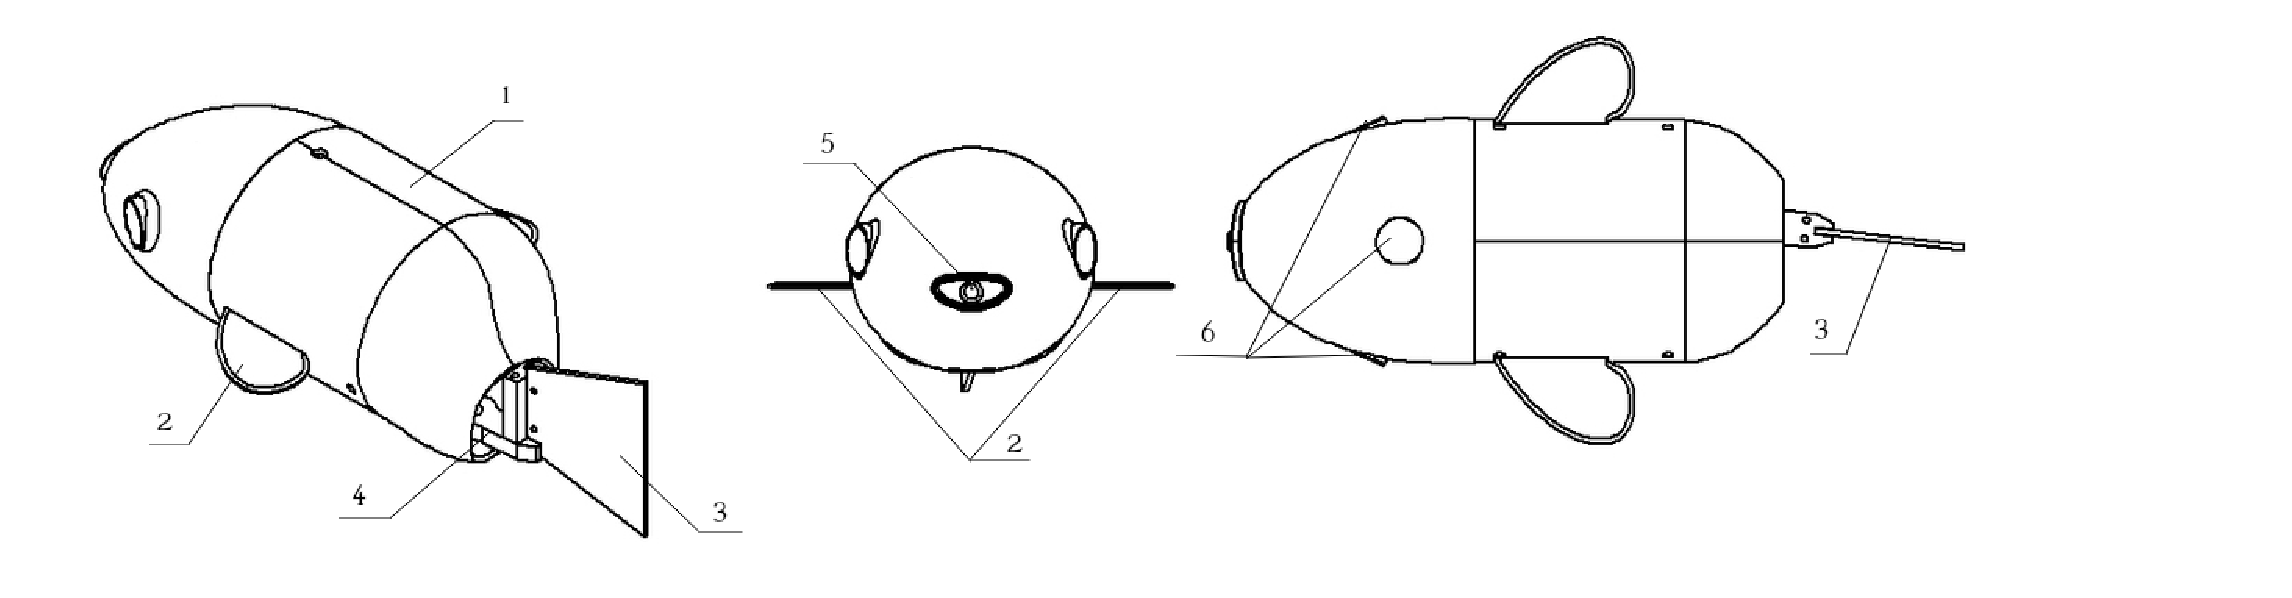
\includegraphics[width=0.95\linewidth]{fig/Fig2.eps}
\caption{CAD model of the robot: 1~--- body with integrated head
fairing; 2~--- pectoral fins (passive stabilizers);
3~--- caudal fin; 4~--- multi-link tail propulsor (5~segments);
5~--- lighting system; 6~--- three cameras.}
\label{fig:cad_model}
\end{figure*}

\clearpage

\begin{figure*}[t!]
\setcaptionmargin{5mm}
\onelinecaptionstrue
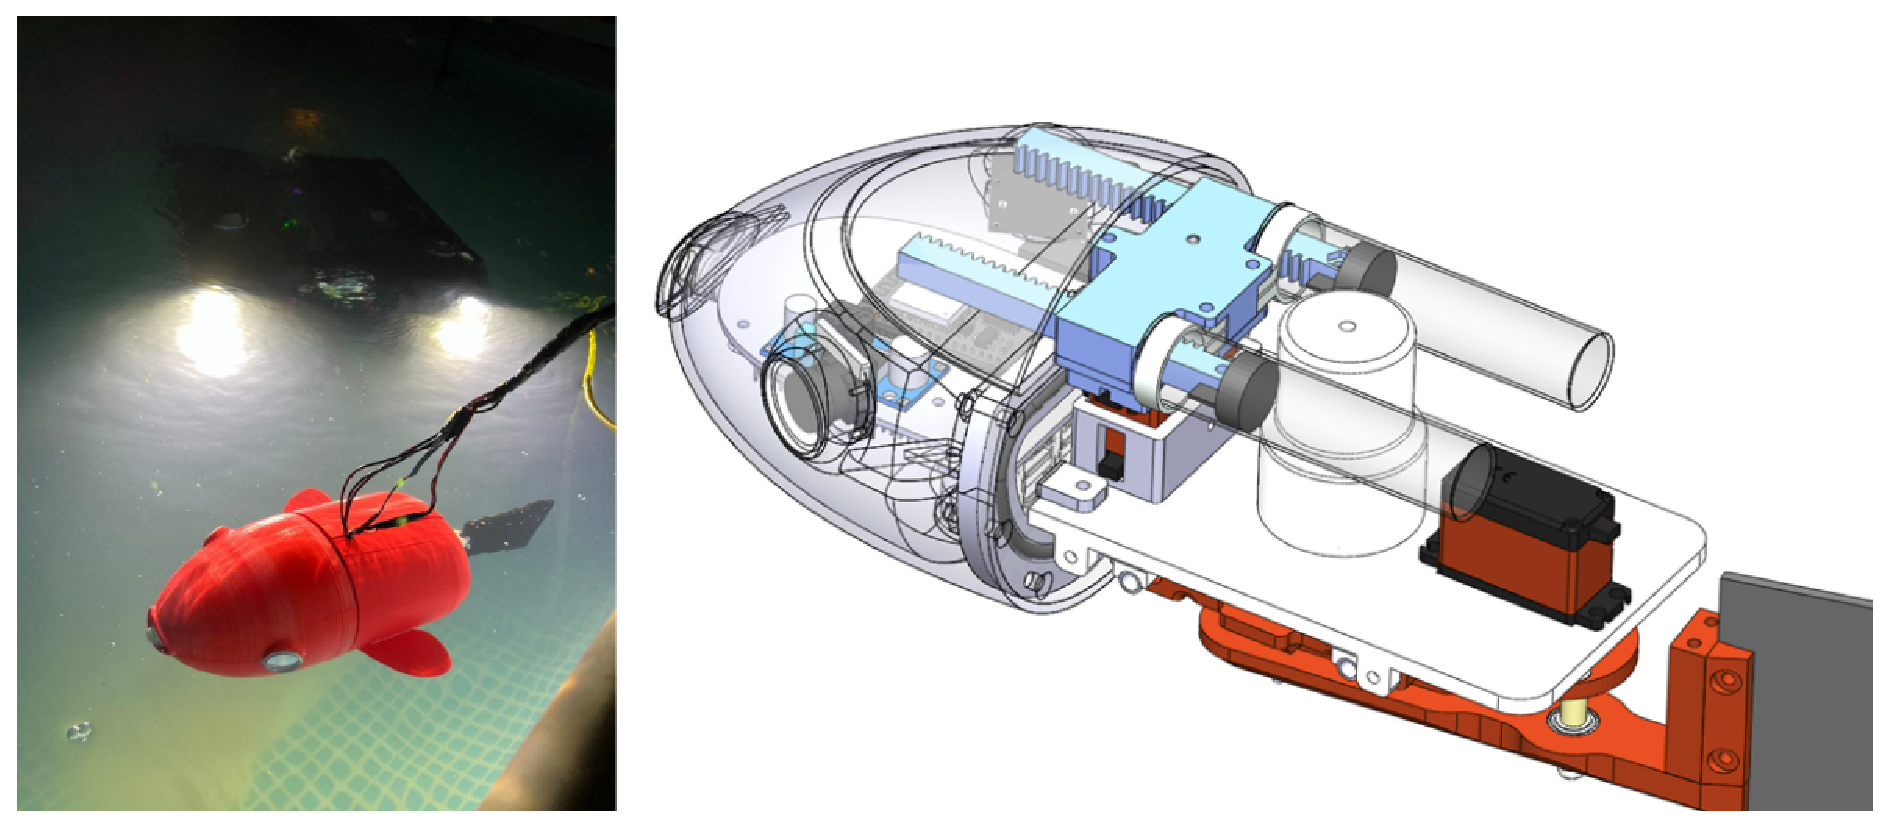
\includegraphics[width=0.95\linewidth]{fig/Fig3.eps}
\caption{Prototype testing and internal structure of the robot.}
\label{fig:prototype}
\end{figure*}

\clearpage

\begin{figure*}[t!]
\setcaptionmargin{5mm}
\onelinecaptionstrue
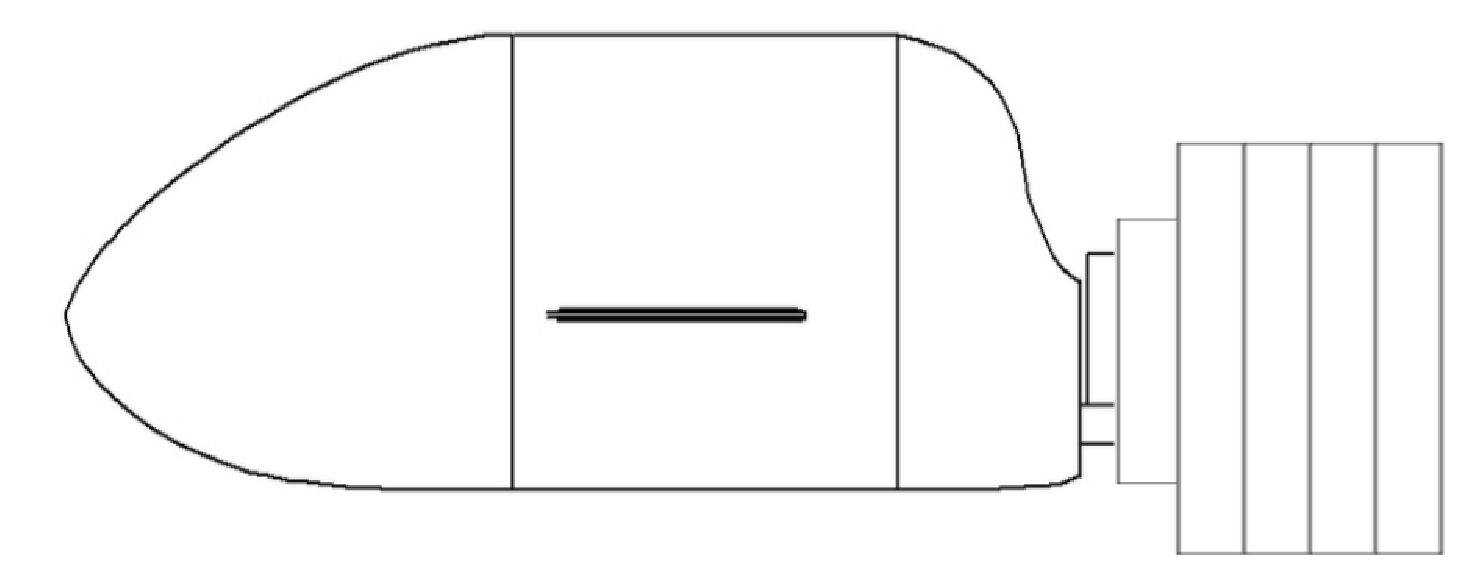
\includegraphics[width=0.95\linewidth]{fig/Fig4.eps}
\caption{Five-segment tail of the robotic fish.}
\label{fig:tail}
\end{figure*}

\clearpage

\begin{figure*}[t!]
\setcaptionmargin{5mm}
\onelinecaptionstrue
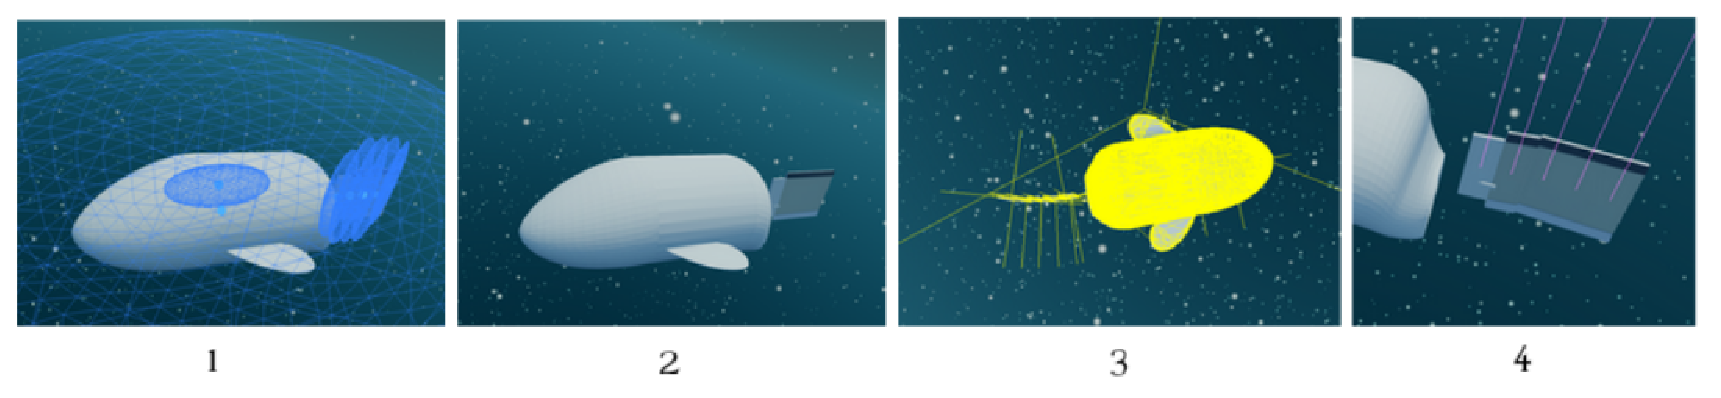
\includegraphics[width=0.95\linewidth]{fig/Fig5.eps}
\caption{Hydrodynamic model, geometric model, collision model,
model of the tail with 5 elements.}
\label{fig:sim_models}
\end{figure*}

\clearpage

\begin{figure*}[t!]
\setcaptionmargin{5mm}
\onelinecaptionstrue
\includegraphics[width=0.95\linewidth]{fig/Fig6.eps}
\caption{Architecture of the developed software.}
\label{fig:architecture}
\end{figure*}

\clearpage

\begin{figure*}[t!]
\setcaptionmargin{5mm}
\onelinecaptionstrue
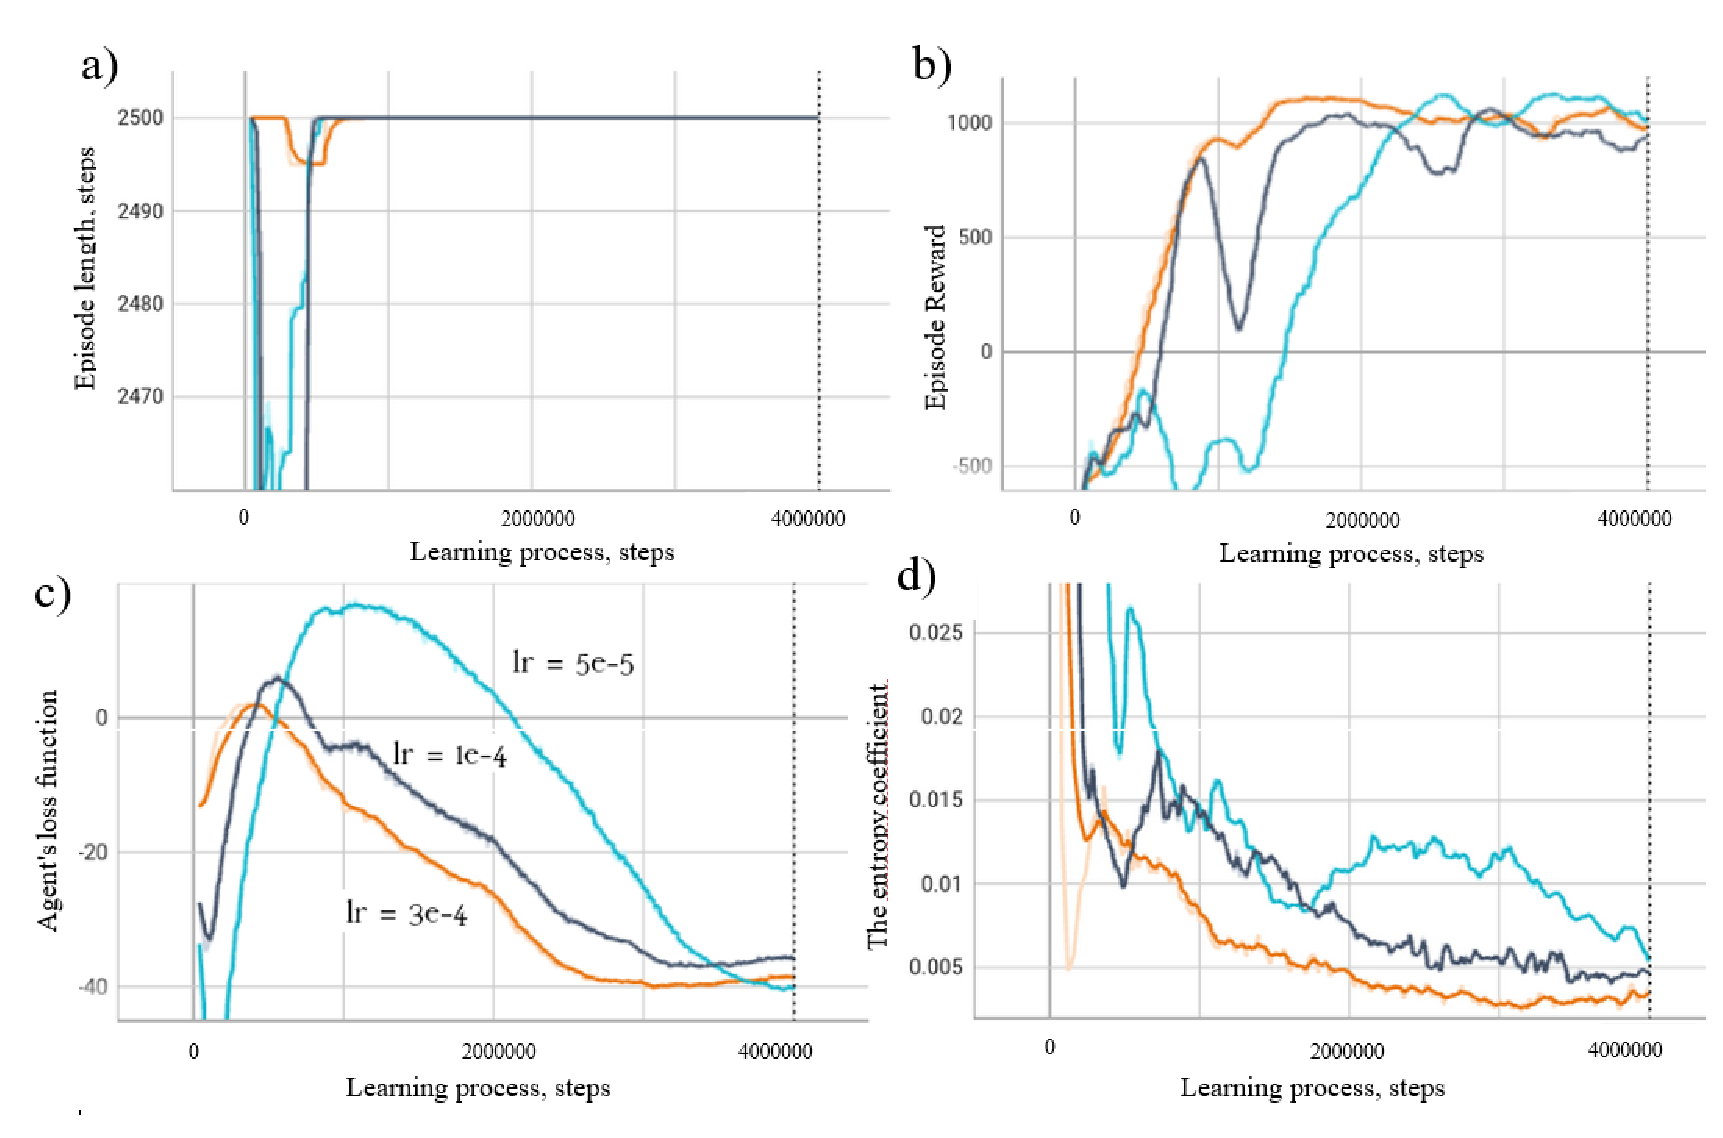
\includegraphics[width=0.95\linewidth]{fig/Fig7.eps}
\caption{(a) Episode length; (b) Total reward per episode;
(c) Agent loss function; (d) Entropy coefficient.}
\label{fig:training_metrics}
\end{figure*}

\clearpage

\begin{figure*}[t!]
\setcaptionmargin{5mm}
\onelinecaptionstrue
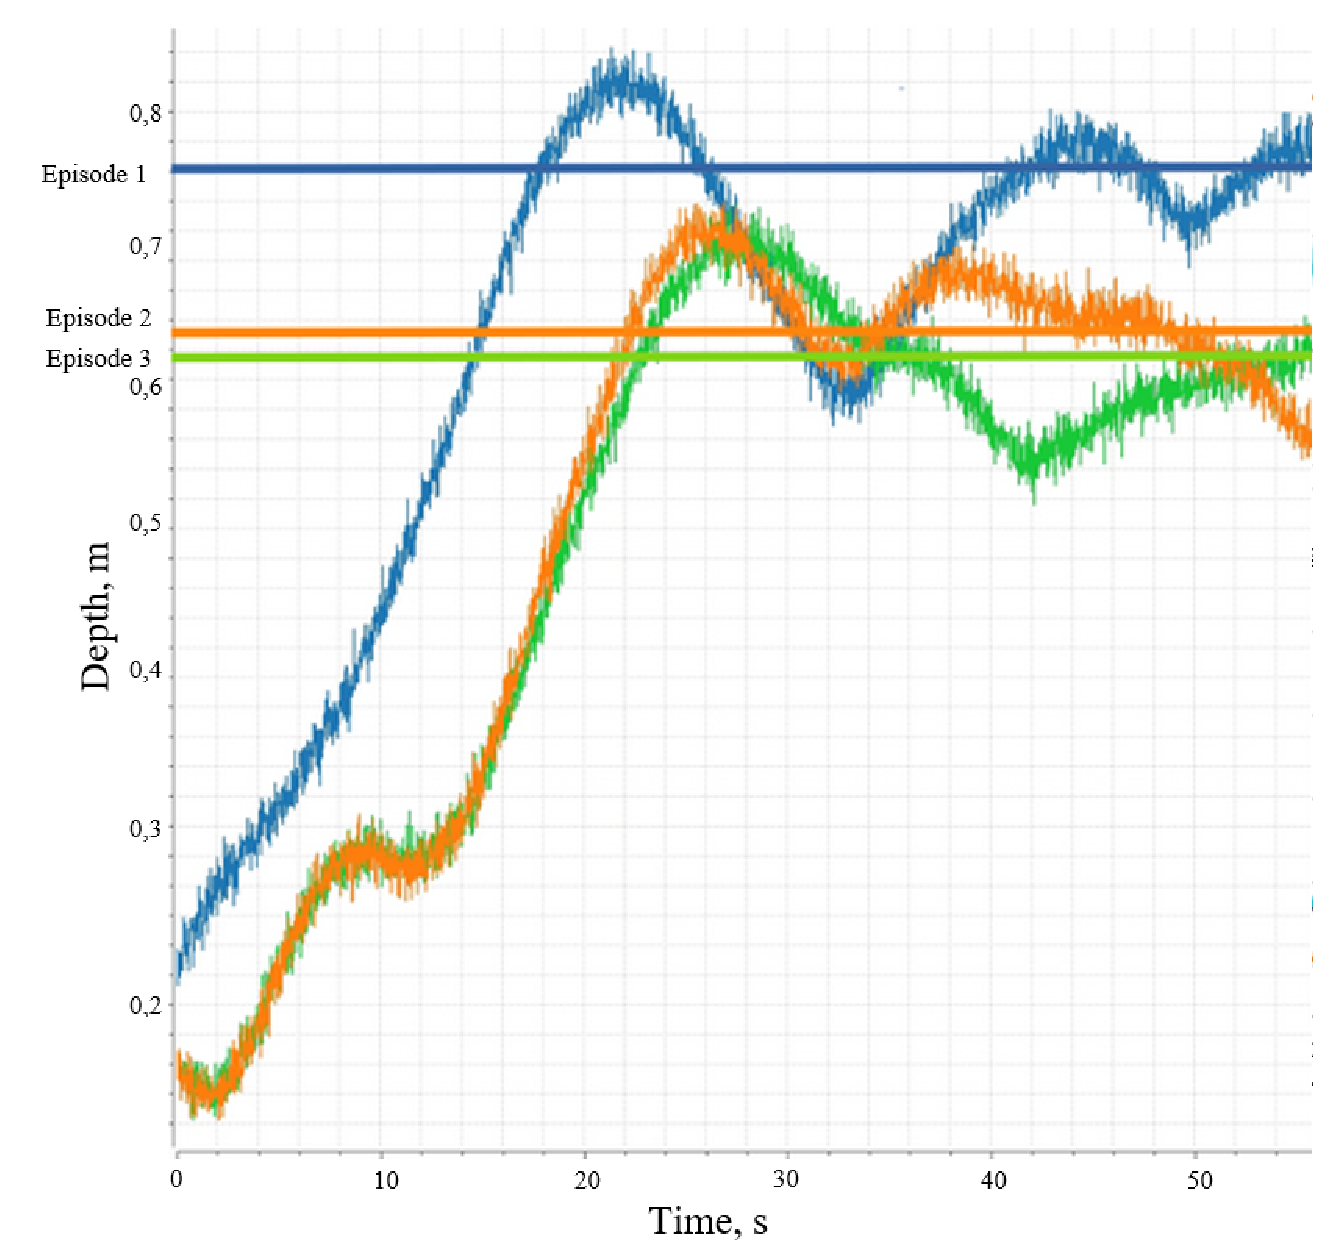
\includegraphics[width=0.95\linewidth]{fig/Fig8.eps}
\caption{Agent depth when using the trained policy for three
different target depths: 0.77~m, 0.65~m, and 0.63~m.}
\label{fig:depth_tracking}
\end{figure*}

% ============== TABLES ==============

\begin{table}
\setcaptionmargin{0mm}
\onelinecaptionstrue
\captionstyle{flushleft}
\caption{Training parameters for the best model}
\label{tab:training_params}
\begin{tabular}{lc}
\hline
Parameter & Value \\
\hline
Number of training steps $N$, steps & 4\,000\,000 \\
Learning rate $lr$ & 3e-04 \\
Discount factor $\gamma$ & 0.99 \\
Replay buffer size $D$, steps & 2\,000\,000 \\
Batch size & 256 \\
Target entropy $H_{\text{target}}$ & $-2.0$ \\
Number of hidden layers & 2 \\
Hidden layer size & 256 \\
Activation function & ReLU \\
Observation buffer length & 5 \\
Entropy coefficient $\alpha$ & automatic \\
Number of parallel training environments & 16--64 \\
\hline
\end{tabular}
\end{table}

\clearpage

\begin{table}
\setcaptionmargin{0mm}
\onelinecaptionstrue
\captionstyle{flushleft}
\caption{Quantitative assessment of the depth control policy quality}
\label{tab:quantitative_metrics}
\begin{tabular}{lc}
\hline
Metric & Value \\
\hline
Steady-state depth error & 0.07 m \\
Standard deviation & 0.04 m \\
Time to enter $\pm 5\%$ zone & 18.5 s \\
Settling time & 22.0 s \\
Maximum velocity (over 10 seconds) & 0.15 m/s \\
Heading hold & 0$^\circ$ \\
\hline
\end{tabular}
\end{table}

\end{document}